\documentclass[letterpaper, 12pt]{article}
\usepackage[english]{babel}
\usepackage{graphicx}

\begin{document}

\begin{titlepage}
\centering
	{\LARGE RoboJackets IGVC}\\
	\vspace{1cm}
	{\Large IGVC Motor and Light Control Board 2017}\\
	\vspace{1cm}
	{\Large Xu, Ruoyang 'Alex' \par}
	\vfill
	{\large Created at November 18, 2017}\\
	\vspace{1cm}
	{\large Last Edited at \today\par}
\end{titlepage}

\tableofcontents
\pagebreak

\section{Overview}
This document explained the function of the Motor and Light Control Board (referred as \emph{motor board} in the following) on \textbf{RoboJackets} IGVC subteam robot \textbf{Jenni} in year 2017 - 2018 and showed how the board is designed with regards to its need, capability and limitation. This document is created in the hope that future developers can have a good understanding of the robot without unnecessary effort. \vspace{6pt}\\
The motor board is the interface between Jenni's software control and her electrical system. IGVC software team completes path-planning on the two onboard Intel NUC computing units and will send command to the motor board. The motor board will then tune the value according to PID tuner and resend it to the motor controller, which will then power the motor.\\
\begin{figure}[h]
\centering
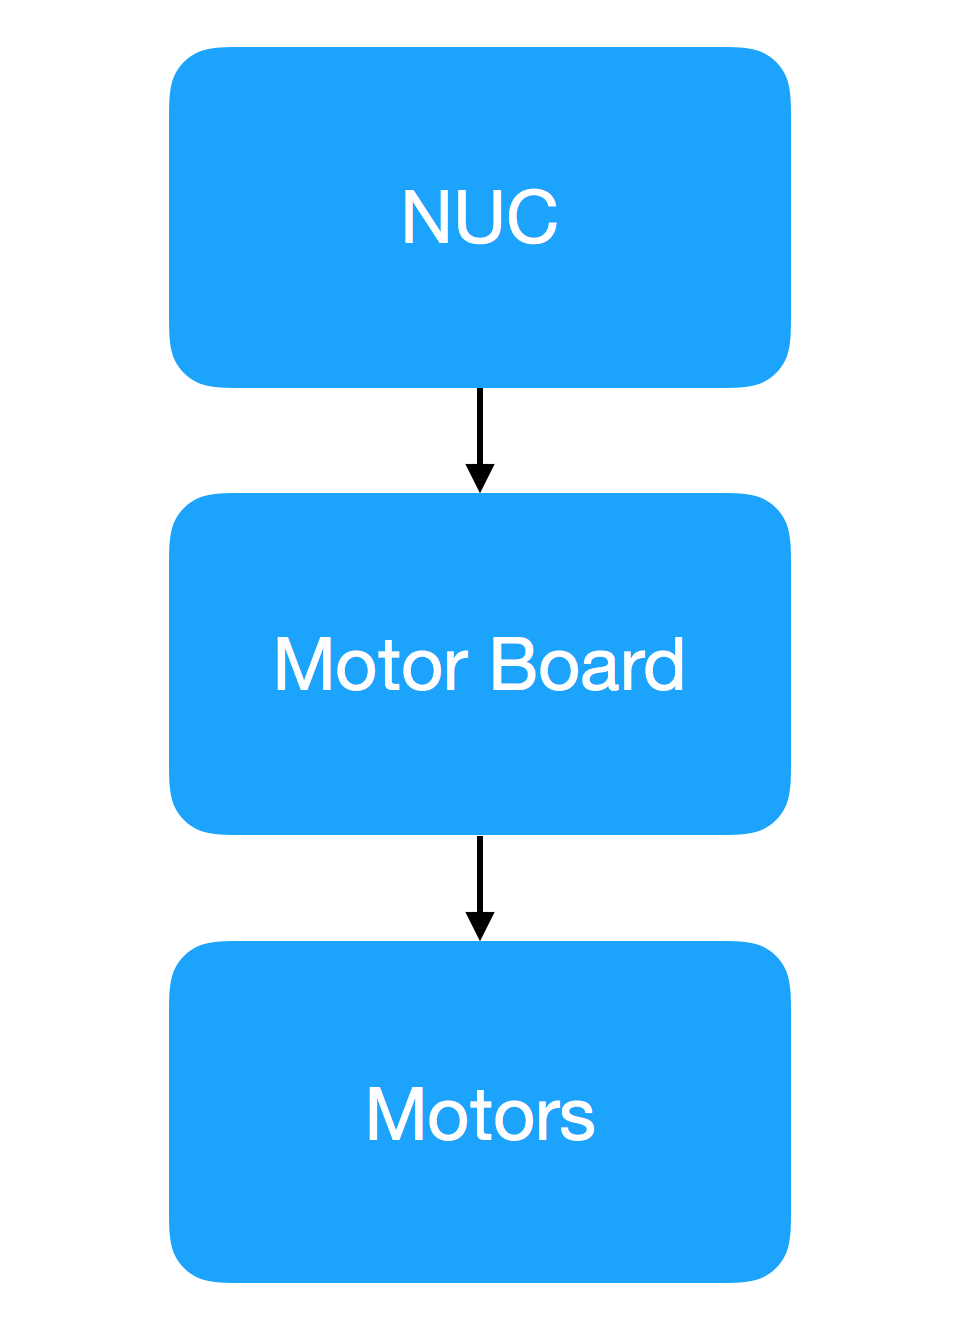
\includegraphics[width=0.5\textwidth]{UpandLow.png}
\caption{Motor Board's Data Input and Output}
\end{figure}

The primary function of the motor board is to ensure the DC motor is operating at the speed given by the NUCs. Secondary functions include controlling the LED under-glow and monitor battery voltage. Circuits supporting each function are entirely separated from each other with the exception that they share the same micro-controller unit and power source.\vspace{6pt}\\
The motor board is controlled by a 

\section{Design of the board}
\subsection{Controlling Unit}
\subsection{Motor Control Circuit}
Subsection of motor control circuit 
\pagebreak
\subsection{Light Control Circuit}
Subsection of light control circuit
\pagebreak
\subsection{Power System}
Subsection of how the system is considered in regard to the power system as well as how the board functions.
\pagebreak
\subsection{Board Layout}
Explanation of how the board is laid out, details including components not covered in schematics.
\pagebreak

\section{Function of the Board}
\subsection{Controlling the board}
\pagebreak
\subsection{Interacting with Peripheral Devices}
\pagebreak

\section{Miscellaneous}
\subsection{Legacy Interfaces}
\pagebreak
\subsection{Expected Future Usage}
\pagebreak

\section{Special Regards}
\pagebreak
\end{document}